\documentclass[lang=cn,10pt]{elegantbook}
\usepackage{gnuplot-lua-tikz}
%\usepackage[active,tightpage]{preview}
%\PreviewEnvironment{tikzpicture}
%\setlength\PreviewBorder{\gpbboxborder}
\usepackage{tikz}
\usepackage{pgfplots}
\usepackage{enumitem}
\pgfplotsset{width=10cm,compat=1.9}
\usepgfplotslibrary{patchplots}
\usetikzlibrary{arrows,calc,decorations.markings,math,arrows.meta}
% We will externalize the figures
\usepgfplotslibrary{external}
\tikzexternalize

\makeatletter
\pgfmathdeclarefunction{myatan2}{2}{%
\begingroup%
  \pgfmathfloattofixed{#1}\edef\tempa{\pgfmathresult}%
  \pgfmathfloattofixed{#2}%
  \pgfkeys{pgf/fpu=false}%
  \pgfmathparse{atan2(\tempa,\pgfmathresult)}\pgfkeys{/pgf/fpu}%
  \pgfmathfloatparsenumber{\pgfmathresult}%
  \pgfmath@smuggleone\pgfmathresult%
\endgroup
}
\makeatother

\begin{document}

\chapter{频率法}

\section{频率特性}

\subsection{传递函数的频率特性}

已知传递函数或信号具有如下频率特性

\begin{equation}
	G(j\omega)=A(\omega)e^{j\phi(\omega)}
\end{equation}

其中频率特性为传递函数中以$j\omega$替换$s$的结果

\begin{equation}
	G(j\omega)=G(s)\Big |_{s=j\omega}=|G(j\omega)|e^{jargG(j\omega)}
\end{equation}

可以得到

\begin{equation}
	\varphi(\omega)=arg{G(j\omega)}
\end{equation}
\begin{equation}
	A(j\omega)=|G(j\omega)|
\end{equation}

\example

设有如下传递函数

\begin{equation}
	G(j\omega)=\frac{1}{1+j\omega\tau}
\end{equation}

求其幅值和相角。

\begin{solution}

	幅值为

	\begin{equation}
		A(\omega)=|G(j\omega)|=\frac{1}{\sqrt{1+\tau^2\omega^2}}
	\end{equation}

	相角为

	\begin{equation}
		\varphi(\omega)=argG(j\omega)=-\arctan{\tau\omega}
	\end{equation}


\end{solution}

\proof

设系统传递函数为

\begin{equation}
	G(s)=\frac{C(s)}{R(s)}=\frac{b_0s^m+\ldots+b_m}{a_0s^n+\ldots+b_m}
\end{equation}

求解该系统在$r(t)=A_r\sin{\omega t}$输入下的动态过程,$C(s)$为像函数

输入信号的拉氏变换为

\begin{equation}
	R(s)=\frac{A_r\omega}{s^2+\omega^2}
\end{equation}

代入

\begin{equation}
	C(s)=G(s)R(s)=\frac{b_0s^m+\ldots+b_m}{a_0s^n+\ldots+b_m}\cdot\frac{A_r\omega}{s^2+\omega^2}
\end{equation}

因式分解

\begin{equation}
	C(s)=\sum_{i=1}^{n}\frac{C_i}{s-s_i}+(\frac{B}{s+j\omega}+\frac{D}{s-j\omega})
\end{equation}

后面两项是系统输出的稳态分量,使用待定系数法求出$B$和$D$

\begin{equation}
	\begin{aligned}
		B & =G(s)\cdot\frac{A_r\omega}{s^2+\omega^2}(s+j\omega)\Big|_{s=-j\omega}     \\
		  & =\frac{|G(j\omega)|}{2}\cdot A_r\cdot e^{-j(argG(j\omega)-\frac{\pi}{2})}
	\end{aligned}
\end{equation}

同理

\begin{equation}
	D=\frac{|G(j\omega)|}{2}\cdot A_r\cdot e^{+j(argG(j\omega)-\frac{\pi}{2})}
\end{equation}

得

\begin{equation}
	\begin{aligned}
		C_s(t) & =\frac{|G(j\omega)|}{2}\cdot A_r\cdot (e^{-j(\omega t+argG(j\omega)-\frac{\pi}{2})}+e^{+j(\omega t+argG(j\omega)-\frac{\pi}{2})})
		\\&=A_c\sin{(\omega t+\varphi)}
	\end{aligned}
\end{equation}

可得

\begin{quote}

	\indent 振幅:$A_c=|G(j\omega)|\cdot A_r$

	\indent 相角:$\omega t+\varphi=\omega t+argG(j\omega)$

\end{quote}

则有

\begin{quote}

	\indent 振幅比(幅频特性):$A(\omega)=\frac{A_c}{A_r}=|G(j\omega)|=|G(s)|\Big|_{s=j\omega}$

	\indent 相位差(相频特性):$\varphi(\omega)=(\omega t+argG(j\omega))-\omega t=argG(j\omega)=argG(s)\Big|_{s=j\omega}$

\end{quote}

得系统的幅相特性

\begin{equation}
	|G(j\omega)|e^{jargG(j\omega)}=A(\omega)e^{j\varphi(\omega)}=G(j\omega)=G(s)\Big|_{s=j\omega}
\end{equation}

注意以上只适用于线性定常系统

\subsection{幅相频率特性}

幅相频率特性可以使用一些曲线描绘出来

\begin{enumerate}

	\item Nyquist(奈奎斯特)曲线:由复函数$G(j\omega)=A(\omega)e^{j\varphi(\omega)}$, 可以分离复函数$G(j\omega)=P(\omega)+jQ(\omega)$  在复平面上绘制

	\item Bode(伯德)图:在对数坐标图上绘制两个图形

	      Bode 图分为对数幅频特性曲线和对数相频特性曲线,

	      对于对数幅频特性曲线:

	      \begin{equation}
		      L(\omega)=20\log|G(j\omega)|=20\log A(\omega)\quad[dB]
	      \end{equation}

	      \begin{tikzpicture}
		      \begin{axis}[width=10cm,height=7cm,
				      axis lines = left,
				      xmode=log,
				      xlabel = \(\omega\),
				      ylabel = {\(L(\omega)\quad[dB]\)},
				      log ticks with fixed point,
				      xmin = 0.1, xmax = 10000,
				      ymin = -20, ymax = 60,
				      xtick = {0.1,1,10,100,1000,10000},
				      ytick = {-20,0,20,40,60},
				      legend pos=north west,
				      ymajorgrids=true,
				      grid style=dashed,
			      ]
		      \end{axis}
	      \end{tikzpicture}

	      \begin{tikzpicture}
		      \begin{axis}[width=10cm,height=7cm,
				      axis lines = left,
				      xmode=log,
				      xlabel = \(\omega\),
				      ylabel = {\(\varphi(\omega)\quad[^\circ]\)},
				      log ticks with fixed point,
				      xmin = 0.1, xmax = 10000,
				      ymin = -270, ymax = 90,
				      xtick = {0.1,1,10,100,1000,10000},
				      ytick distance=90 ,
				      legend pos=north west,
				      ymajorgrids=true,
				      grid style=dashed,
			      ]
		      \end{axis}
	      \end{tikzpicture}

\end{enumerate}

\section{基本环节的频率特性}

\subsection{比例环节}

该环节传递函数为

\begin{equation}
	G(s)=K
\end{equation}

\begin{itemize}

	\item{

	            其 Nyquist 曲线是复平面上的一个点

	            \begin{equation}
		            G(j\omega)=K
	            \end{equation}

	            \begin{center}
		            \begin{tikzpicture}
			            \begin{axis}[width = 5cm, height = 5cm,
					            axis lines = center,
					            xlabel = \(1\), ylabel = \(i\),
					            xmin = -1, xmax = 1,
					            ymin = -1, ymax = 1,
					            xticklabel = \empty, yticklabel = \empty,
				            ]
				            \addplot+ [color=red] coordinates {
						            (0.5,0)
					            };
				            \node [above] at (axis cs: 0.5, 0) {$K$};
			            \end{axis}
		            \end{tikzpicture}
	            \end{center}

	      }

	\item{

	            其 Bode 图求解得

	            \begin{equation}
		            L(\omega)=20\log{K}
	            \end{equation}
	            \begin{equation}
		            \varphi(\omega)=0
	            \end{equation}

	            \begin{center}
		            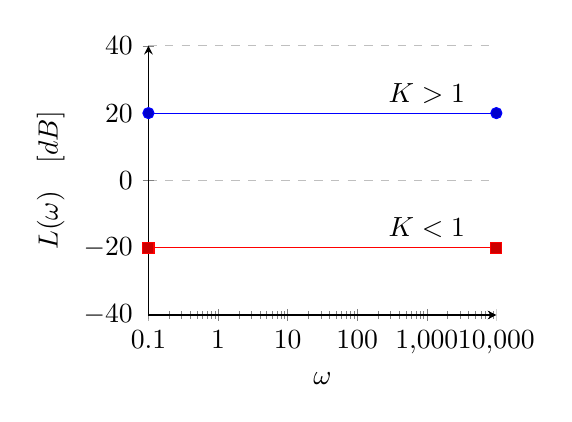
\begin{tikzpicture}
			            \begin{axis}[width=6cm,height=5cm,
					            axis lines = left,
					            xmode = log,
					            xlabel = \(\omega\), ylabel = {\(L(\omega)\quad[dB]\)},
					            log ticks with fixed point,
					            xmin = 0.1, xmax = 10000,
					            ymin = -40, ymax = 40,
					            xtick = {0.1,1,10,100,1000,10000},
					            ytick distance = 20,
					            legend pos=north west,
					            ymajorgrids=true,
					            grid style=dashed,
				            ]
				            \addplot coordinates {
						            (0.1,20)(10000,20)
					            };
				            \node [above] at (axis cs: 1000, 20) {$K>1$};
				            \addplot coordinates {
						            (0.1,-20)(10000,-20)
					            };
				            \node [above] at (axis cs: 1000, -20) {$K<1$};
			            \end{axis}
		            \end{tikzpicture}
		            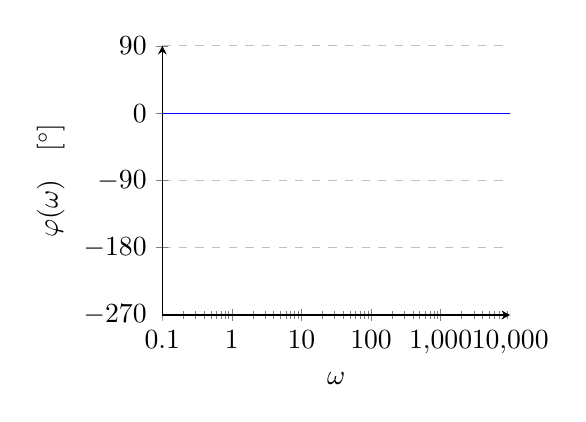
\begin{tikzpicture}
			            \begin{axis}[width=6cm,height=5cm,
					            axis lines = left,
					            xmode=log,
					            xlabel = \(\omega\), ylabel = {\(\varphi(\omega)\quad[^\circ]\)},
					            log ticks with fixed point,
					            xmin = 0.1, xmax = 10000,
					            ymin = -270, ymax = 90,
					            xtick = {0.1,1,10,100,1000,10000},
					            ytick distance = 90,
					            legend pos=north west,
					            ymajorgrids=true,
					            grid style=dashed,
				            ]
				            \addplot [
					            domain=0.1:10000,
					            samples=200,
					            color=blue,
				            ] { 0 * x };
			            \end{axis}
		            \end{tikzpicture}
	            \end{center}
	      }
\end{itemize}

\subsection{惯性环节}

该环节传递函数为

\begin{equation}
	G(s)=\frac{1}{Ts+1}
\end{equation}

\begin{itemize}
	\item{ 其 Nyquist 图像是一个半圆
	            \begin{equation}
		            G(j\omega)=\frac{1}{j\omega T+1}=\frac{1}{\sqrt{1+T^2\omega^2}}e^{j(-\arctan{T\omega})}=\frac{1}{1+T^2\omega^2}+j\frac{-T\omega}{1+T^2\omega^2}
	            \end{equation}

	            \begin{center}
		            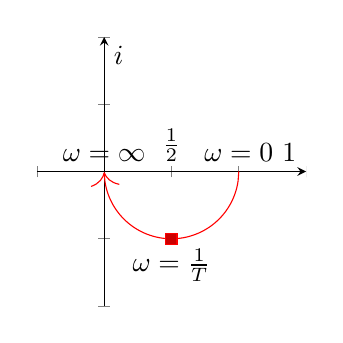
\begin{tikzpicture}
			            \begin{axis}[width=5cm,height=5cm,
					            axis lines = center,
					            xlabel = \(1\), ylabel = \(i\),
					            xmin = -0.5, xmax = 1.5,
					            ymin = -1, ymax = 1,
					            xticklabel=\empty, yticklabel=\empty,
				            ]
				            \addplot [
				            domain = 1:0,
				            color = red,
				            samples = 200,
				            -{>[scale = 2.0]},
				            ] { -sqrt(0.25-((1-x)-0.5)^2) };
				            \node [above] at (axis cs: 0.5, 0) {$\frac{1}{2}$};
				            \node [above] at (axis cs: 1, 0) {$\omega=0$};
				            \addplot+ [color=red] coordinates {
						            (0.5,-0.5)
					            };
				            \node [below] at (axis cs: 0.5, -0.5) {$\omega=\frac{1}{T}$};
				            \node [above] at (axis cs: 0, 0) {$\omega=\infty$};
			            \end{axis}
		            \end{tikzpicture}
	            \end{center}
	      }

	\item{ 其 Bode 图求解得,具有低通滤波特性,且输出相位滞后于输入信号相位

	            \begin{equation}
		            L(\omega)=20\log{\frac{1}{\sqrt{1+T^2\omega^2}}}=-20\log{\sqrt{1+T^2\omega^2}}
	            \end{equation}
	            \begin{equation}
		            \varphi(\omega)=-\arctan{T\omega}
	            \end{equation}

	            使用近似画法进行绘制(蓝线),对比精确结果(红线),在$\omega=\frac{1}{T}$处误差为-3dB。

	            \begin{center}
		            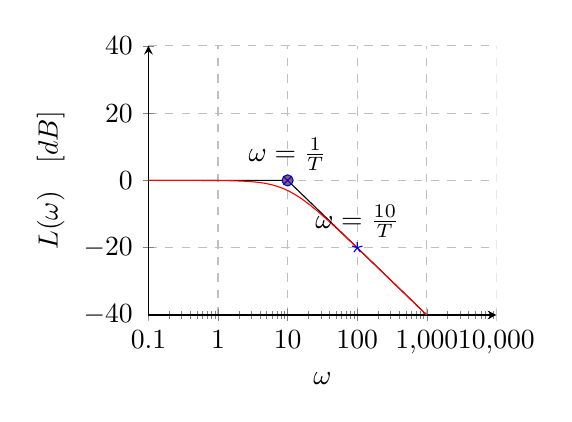
\begin{tikzpicture}
			            \begin{axis}[width = 6cm, height = 5cm,
					            axis lines = left,
					            xmode = log,
					            xlabel = \(\omega\), ylabel = {\(L(\omega)\quad[dB]\)},
					            log ticks with fixed point,
					            xmin = 0.1, xmax = 10000,
					            ymin = -40, ymax = 40,
					            xtick = {0.1,1,10,100,1000,10000},
					            ytick distance = 20,
					            legend pos = north west,
					            ymajorgrids = true,
					            xmajorgrids = true,
					            grid style = dashed,
				            ]
				            \addplot [
					            mark=\empty,
				            ] coordinates {
						            (0.1,0)(10,0)(1000,-40)
					            };
				            \addplot [
					            domain=0.1:10000,
					            samples=200,
					            color=red,
				            ] { - 20 * log10( sqrt( 1 + ( x / 10 )^2 ) ) };
				            % \addplot [] {20*log(10,x)};
				            \addplot+ [color=blue] coordinates {
						            (10,0)
					            };
				            \node [above] at (axis cs: 10, 0) {$\omega=\frac{1}{T}$};
				            \addplot+ [color=blue] coordinates {
						            (100,-20)
					            };
				            \node [above] at (axis cs: 100, -20) {$\omega=\frac{10}{T}$};
			            \end{axis}
		            \end{tikzpicture}
		            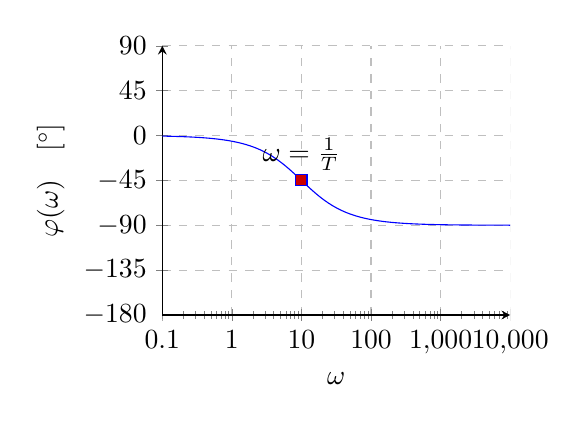
\begin{tikzpicture}
			            \begin{axis}[width=6cm,height=5cm,
					            axis lines = left,
					            xmode = log,
					            xlabel = \(\omega\), ylabel = {\(\varphi(\omega)\quad[^\circ]\)},
					            log ticks with fixed point,
					            xmin = 0.1, xmax = 10000,
					            ymin = -180, ymax = 90,
					            xtick = {0.1,1,10,100,1000,10000},
					            ytick distance = 45,
					            legend pos = north west,
					            ymajorgrids = true,
					            xmajorgrids = true,
					            grid style = dashed,
				            ]
				            \addplot [
					            domain=0.1:10000,
					            samples=200,
					            color=blue,
				            ] { - atan( x / 10 ) };
				            \addplot+ [color=blue] coordinates {
						            (10,-45)
					            };
				            \node [above] at (axis cs: 10, -45) {$\omega=\frac{1}{T}$};
			            \end{axis}
		            \end{tikzpicture}
	            \end{center}
	      }
\end{itemize}

\subsection{积分环节}

该环节具有如下传递函数:

\begin{equation}
	G(s)=\frac{1}{s}
\end{equation}

\begin{itemize}
	\item{ 其 Nyquist 图像是一条趋向原点的直线,其幅值与$\omega$成反比

	            \begin{equation}
		            G(j\omega)=\frac{1}{j\omega}=\frac{1}{\omega}e^{-j\frac{\pi}{2}}=0-j\frac{1}{\omega}
	            \end{equation}

	            \begin{center}
		            \begin{tikzpicture}
			            \begin{axis}[width=5cm,height=5cm,
					            axis lines = center,
					            xlabel = \(1\), ylabel = \(i\),
					            xmin = -0.5, xmax = 1.5,
					            ymin = -1, ymax = 1,
					            xticklabel=\empty, yticklabel=\empty,
				            ]
				            \addplot [
				            color = red,
				            -{>[scale = 2.0]},
				            mark=\empty,
				            ] coordinates {
						            (0,-1)(0,0)
					            };
				            \node [right] at (axis cs: 0, -0.4) {$\omega\rightarrow\infty$};
			            \end{axis}
		            \end{tikzpicture}
	            \end{center}
	      }
	\item{ 其 Bode 图如下,

	            \begin{equation}
		            L(\omega)=20\log{\frac{1}{\omega}}=-20\log{\omega}
	            \end{equation}
	            \begin{equation}
		            \varphi(\omega)=-\frac{\pi}{2}
	            \end{equation}

	            \begin{center}
		            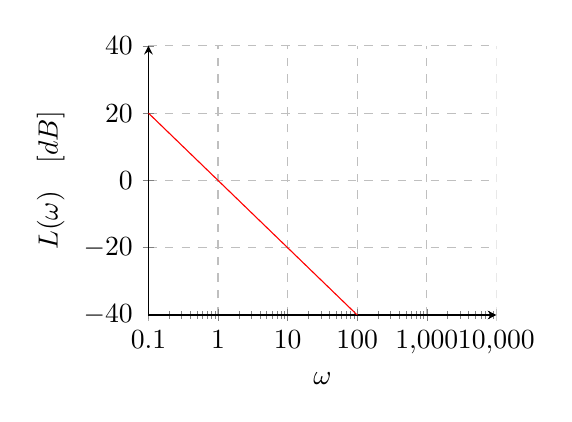
\begin{tikzpicture}
			            \begin{axis}[width = 6cm, height = 5cm,
					            axis lines = left,
					            xmode = log,
					            xlabel = \(\omega\), ylabel = {\(L(\omega)\quad[dB]\)},
					            log ticks with fixed point,
					            xmin = 0.1, xmax = 10000,
					            ymin = -40, ymax = 40,
					            xtick = {0.1,1,10,100,1000,10000}, ytick distance = 20,
					            legend pos = north west,
					            ymajorgrids = true,
					            xmajorgrids = true,
					            grid style = dashed,
				            ]
				            \addplot [
					            domain=0.1:10000,
					            samples=200,
					            color=red,
				            ] { - 20 * log10( x ) };

			            \end{axis}
		            \end{tikzpicture}
		            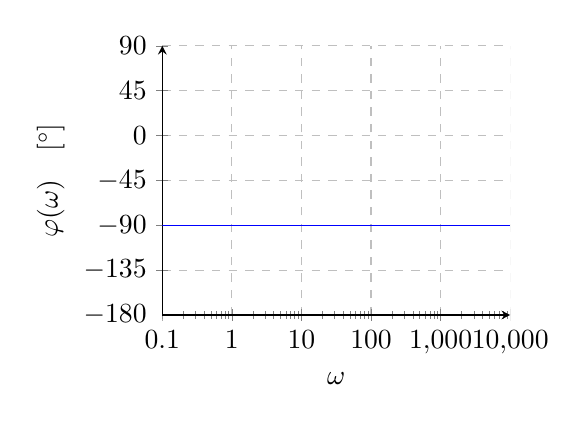
\begin{tikzpicture}
			            \begin{axis}[width=6cm,height=5cm,
					            axis lines = left,
					            xmode = log,
					            xlabel = \(\omega\), ylabel = {\(\varphi(\omega)\quad[^\circ]\)},
					            log ticks with fixed point,
					            xmin = 0.1, xmax = 10000,
					            ymin = -180, ymax = 90,
					            xtick = {0.1,1,10,100,1000,10000}, ytick distance = 45,
					            legend pos = north west,
					            ymajorgrids = true,
					            xmajorgrids = true,
					            grid style = dashed,
				            ]
				            \addplot [
					            domain=0.1:10000,
					            samples=200,
					            color=blue,
				            ] { -90 };

			            \end{axis}
		            \end{tikzpicture}
	            \end{center}
	      }
\end{itemize}

\subsection{震荡环节}

该环节有以下传递函数

\begin{equation}
	G(s)=\frac{\omega_n^2}{s^2+2\xi\omega_ns+\omega_n^2}=\frac{1}{T^2s^2+2\xi Ts+1}\quad(T=\frac{1}{\omega_n})
\end{equation}

\begin{itemize}
	\item{ 其 Nyquist 图像如下

	            \begin{equation}
		            G(j\omega)=\frac{1}{-T^2\omega^2+j2\xi T\omega+1}=\frac{1}{\sqrt{(1-T^2\omega^2)^2+(2\xi T\omega)^2}}e^{-j\arctan{\frac{2\xi T\omega}{1-T^2\omega^2}}}
	            \end{equation}

	            \begin{center}
		            \begin{tikzpicture}
			            \begin{axis}[width=5cm,height=5cm,
					            axis lines = center,
					            xlabel = \(1\), ylabel = \(i\),
					            xmin = -0.5, xmax = 1.5,
					            ymin = -1.5, ymax = 0.5,
					            xticklabel = \empty, yticklabel = \empty,
				            ]
				            \addplot [
				            mark=\empty,
				            -{>[scale = 2.0]},
				            patch,
				            patch type=bezier spline,
				            color = red,
				            ] coordinates {
						            (1,0)(0,0)(0,-1.5)(-1,-0.5)
					            };
				            \node [right] at (axis cs: 0, -0.4) {$\xi=0.6$};
			            \end{axis}
		            \end{tikzpicture}
	            \end{center}
	      }

	\item{ 其 Bode 图如下,

	            \begin{equation}
		            L(\omega)=20\log{\frac{1}{\sqrt{(1-T^2\omega^2)^2+(2\xi T\omega)^2}}}=-20\log{\sqrt{(1-T^2\omega^2)^2+(2\xi T\omega)^2}}
	            \end{equation}
	            \begin{equation}
		            \varphi(\omega)=-\arctan{\frac{2\xi T\omega}{1-T^2\omega^2}}
	            \end{equation}

	            \begin{center}
		            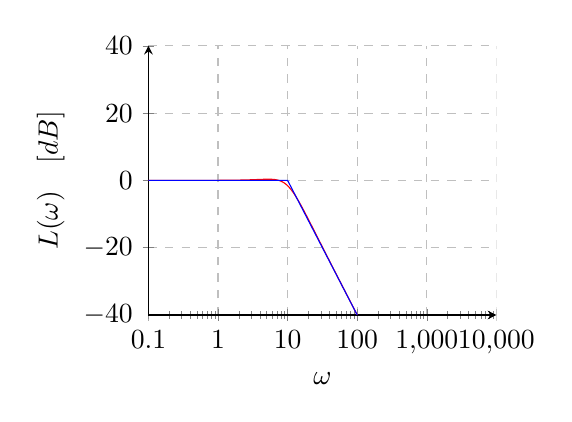
\begin{tikzpicture}
			            \begin{axis}[width = 6cm, height = 5cm,
					            axis lines = left,
					            xmode = log,
					            xlabel = \(\omega\), ylabel = {\(L(\omega)\quad[dB]\)},
					            log ticks with fixed point,
					            xmin = 0.1, xmax = 10000,
					            ymin = -40, ymax = 40,
					            xtick = {0.1,1,10,100,1000,10000}, ytick distance = 20,
					            legend pos = north west,
					            ymajorgrids = true,
					            xmajorgrids = true,
					            grid style = dashed,
				            ]
				            \addplot [
					            domain=0.1:10000,
					            samples=200,
					            color=red,
				            ] { - 20 * log10( sqrt( ( 1.0-(x/10)^2 )^2 + ( 2*0.6*x/10 )^2 ) ) };
				            \addplot [
					            color=blue,
					            mark=\empty,
				            ] coordinates {
						            (0.1,0)(10,0)(100,-40)
					            };
			            \end{axis}
		            \end{tikzpicture}
		            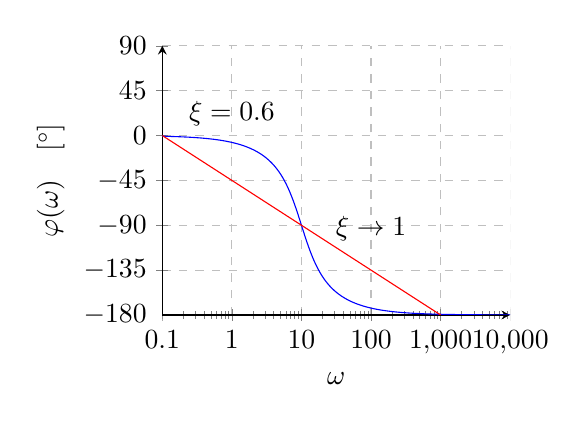
\begin{tikzpicture}
			            \begin{axis}[width=6cm,height=5cm,
					            axis lines = left,
					            xmode = log,
					            xlabel = \(\omega\), ylabel = {\(\varphi(\omega)\quad[^\circ]\)},
					            log ticks with fixed point,
					            xmin = 0.1, xmax = 10000,
					            ymin = -180, ymax = 90,
					            xtick = {0.1,1,10,100,1000,10000}, ytick distance = 45,
					            legend pos = north west,
					            ymajorgrids = true,
					            xmajorgrids = true,
					            grid style = dashed,
				            ]
				            \addplot [
					            domain=0.1:10,
					            domain y= 0:-180,
					            samples=200,
					            color=blue,
				            ] { - atan( ( 2 * 0.6 * x/10 ) / ( 1.0 - ( x/10 )^2 ) ) };
				            \addplot [
					            domain=10.0001:10000,
					            domain y= 0:-180,
					            samples=200,
					            color=blue,
				            ] { - atan( ( 2 * 0.6 * x/10 ) / ( 1.0 - ( x/10 )^2 ) ) - 180 };
				            \node [above] at (axis cs: 1, 0) {$\xi=0.6$};
				            \addplot[
					            color=red,
					            mark=\empty,
				            ] coordinates {(0.1,0)(1000,-180)};
				            \node [above] at (axis cs: 100, -115) {$\xi\rightarrow 1$};
			            \end{axis}
		            \end{tikzpicture}
	            \end{center}
	      }
\end{itemize}

当$\xi<0.707$时,对数幅频特性曲线将出现峰值,令

\begin{equation}
	\frac{\mathrm{d}A(\omega)}{\mathrm{d}\omega}=0
\end{equation}

得

\begin{equation}
	\omega_m=\omega_n\sqrt{1-2\xi^2}
\end{equation}

此时峰值频率和自然频率一致,引起共振。

当$\xi>0.707$时,$\omega_m$无实数值,$L(\omega)$无峰值,呈单调递减。

\subsection{微分环节}

微分环节的传递函数为

\begin{equation}
	G(s)=s
\end{equation}


\begin{itemize}
	\item{ 其 Nyquist 图像如下

	            \begin{equation}
		            G(j\omega)=j\omega=\omega e^{j\frac{\pi}{2}}
	            \end{equation}

	            \begin{center}
		            \begin{tikzpicture}
			            \begin{axis}[width=5cm,height=5cm,
					            axis lines = center,
					            xlabel = \(1\), ylabel = \(i\),
					            xmin = -0.5, xmax = 1.5,
					            ymin = -1, ymax = 1,
					            xticklabel = \empty, yticklabel = \empty,
				            ]
				            \addplot [
				            mark=\empty,
				            -{>[scale = 2.0]},
				            color = red,
				            ] coordinates {
						            (0,0)(0,1)
					            };
				            \node [right] at (axis cs: 0, 0.4) {$\omega\rightarrow\infty$};
			            \end{axis}
		            \end{tikzpicture}
	            \end{center}
	      }

	\item{ 其 Bode 图如下,

	            \begin{gather}
		            L(\omega)=20\log{\omega}\\
		            \varphi(\omega)=\frac{\pi}{2}
	            \end{gather}

	            \begin{center}
		            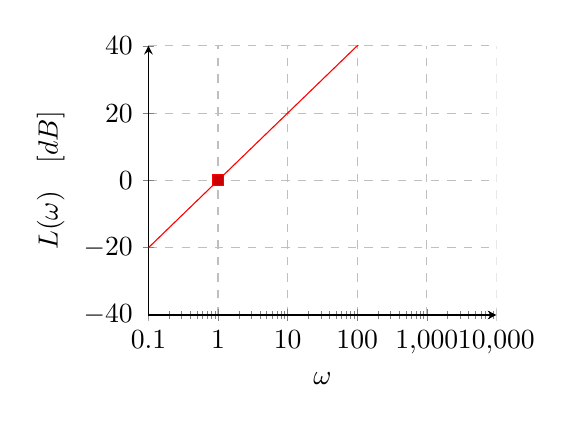
\begin{tikzpicture}
			            \begin{axis}[width = 6cm, height = 5cm,
					            axis lines = left,
					            xmode = log,
					            xlabel = \(\omega\), ylabel = {\(L(\omega)\quad[dB]\)},
					            log ticks with fixed point,
					            xmin = 0.1, xmax = 10000,
					            ymin = -40, ymax = 40,
					            xtick = {0.1,1,10,100,1000,10000}, ytick distance = 20,
					            legend pos = north west,
					            ymajorgrids = true,
					            xmajorgrids = true,
					            grid style = dashed,
				            ]
				            \addplot [
					            domain=0.1:10000,
					            samples=200,
					            color=red,
				            ] { 20 * log10( x ) };
				            \addplot+ [color=red] coordinates {(1,0)};
			            \end{axis}
		            \end{tikzpicture}
		            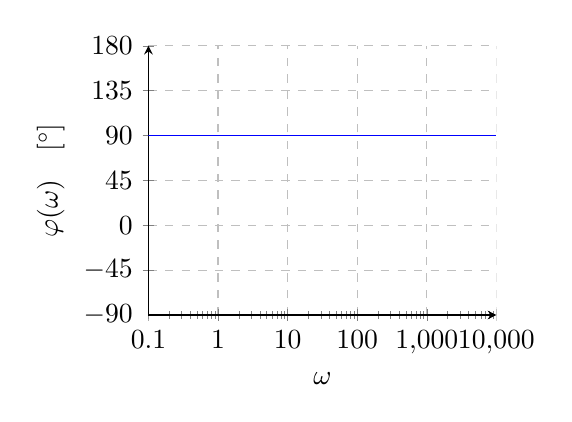
\begin{tikzpicture}
			            \begin{axis}[width=6cm,height=5cm,
					            axis lines = left,
					            xmode = log,
					            xlabel = \(\omega\), ylabel = {\(\varphi(\omega)\quad[^\circ]\)},
					            log ticks with fixed point,
					            xmin = 0.1, xmax = 10000,
					            ymin = -90, ymax = 180,
					            xtick = {0.1,1,10,100,1000,10000}, ytick distance = 45,
					            legend pos = north west,
					            ymajorgrids = true,
					            xmajorgrids = true,
					            grid style = dashed,
				            ]
				            \addplot [
					            domain=0.1:10000,
					            domain y= 0:-180,
					            samples=200,
					            color=blue,
				            ] { 90 };
			            \end{axis}
		            \end{tikzpicture}
	            \end{center}
	      }
\end{itemize}

此外还有一阶微分环节和二阶微分环节

\begin{gather}
	G(j\omega)=1+jT\omega\\
	G(j\omega)=1+2\xi T(j\omega)+T^2(j\omega)^2
\end{gather}

\begin{itemize}
	\item{ 其 Nyquist 图像如下

	            \begin{center}
		            \begin{tikzpicture}
			            \begin{axis}[width=5cm,height=5cm,
					            axis lines = center,
					            xlabel = \(1\), ylabel = \(i\),
					            xmin = -0.5, xmax = 1.5,
					            ymin = -1, ymax = 1,
					            xticklabel = \empty, yticklabel = \empty,
				            ]
				            \addplot [
				            mark=\empty,
				            -{>[scale = 2.0]},
				            color = red,
				            ] coordinates {
						            (1,0)(1,1)
					            };
				            \node [right] at (axis cs: 0, 0.4) {$\omega\rightarrow\infty$};
			            \end{axis}
		            \end{tikzpicture}
		            \begin{tikzpicture}
			            \begin{axis}[width=5cm,height=5cm,
					            axis lines = center,
					            xlabel = \(1\), ylabel = \(i\),
					            xmin = -0.5, xmax = 1.5,
					            ymin = -1, ymax = 1,
					            xticklabel = \empty, yticklabel = \empty,
				            ]
				            \addplot [
				            mark=\empty,
				            -{>[scale = 2.0]},
				            color = red,
				            domain = 1:-0.5,
				            ] {
				            0.5*sqrt(-(x-1))
				            };
				            \node [] at (axis cs: 1, 0.5) {$\omega\rightarrow\infty$};
			            \end{axis}
		            \end{tikzpicture}
	            \end{center}
	      }

	\item{ 他们的 Bode 图如下,与惯性环节相似,关于x轴对称


	            \begin{center}
		            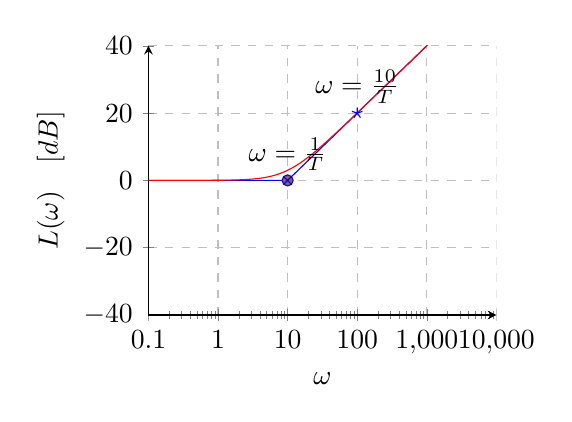
\begin{tikzpicture}
			            \begin{axis}[width = 6cm, height = 5cm,
					            axis lines = left,
					            xmode = log,
					            xlabel = \(\omega\), ylabel = {\(L(\omega)\quad[dB]\)},
					            log ticks with fixed point,
					            xmin = 0.1, xmax = 10000,
					            ymin = -40, ymax = 40,
					            xtick = {0.1,1,10,100,1000,10000},
					            ytick distance = 20,
					            legend pos = north west,
					            ymajorgrids = true,
					            xmajorgrids = true,
					            grid style = dashed,
				            ]
				            \addplot [
					            mark=\empty,
					            color=blue,
				            ] coordinates {
						            (0.1,0)(10,0)(1000,40)
					            };
				            \addplot [
					            domain=0.1:10000,
					            samples=200,
					            color=red,
				            ] { 20 * log10( sqrt( 1 + ( x / 10 )^2 ) ) };
				            % \addplot [] {20*log(10,x)};
				            \addplot+ [color=blue] coordinates {
						            (10,0)
					            };
				            \node [above] at (axis cs: 10, 0) {$\omega=\frac{1}{T}$};
				            \addplot+ [color=blue] coordinates {
						            (100,20)
					            };
				            \node [above] at (axis cs: 100, 20) {$\omega=\frac{10}{T}$};
			            \end{axis}
		            \end{tikzpicture}
		            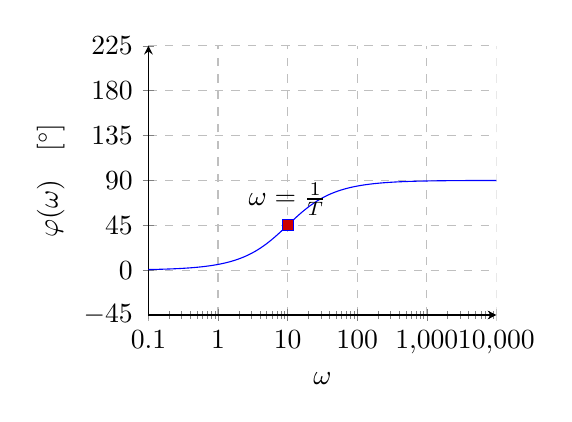
\begin{tikzpicture}
			            \begin{axis}[width=6cm,height=5cm,
					            axis lines = left,
					            xmode = log,
					            xlabel = \(\omega\), ylabel = {\(\varphi(\omega)\quad[^\circ]\)},
					            log ticks with fixed point,
					            xmin = 0.1, xmax = 10000,
					            ymin = -45, ymax = 225,
					            xtick = {0.1,1,10,100,1000,10000},
					            ytick distance = 45,
					            legend pos = north west,
					            ymajorgrids = true,
					            xmajorgrids = true,
					            grid style = dashed,
				            ]
				            \addplot [
					            domain=0.1:10000,
					            samples=200,
					            color=blue,
				            ] { atan( x / 10 ) };
				            \addplot+ [color=blue] coordinates {
						            (10,45)
					            };
				            \node [above] at (axis cs: 10, 45) {$\omega=\frac{1}{T}$};
			            \end{axis}
		            \end{tikzpicture}
	            \end{center}

	            \begin{center}
		            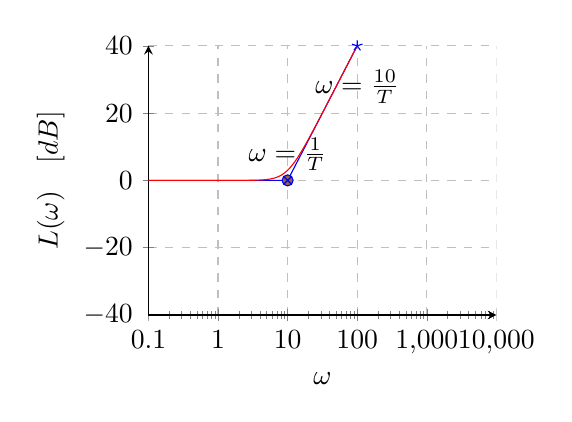
\begin{tikzpicture}
			            \begin{axis}[width = 6cm, height = 5cm,
					            axis lines = left,
					            xmode = log,
					            xlabel = \(\omega\), ylabel = {\(L(\omega)\quad[dB]\)},
					            log ticks with fixed point,
					            xmin = 0.1, xmax = 10000,
					            ymin = -40, ymax = 40,
					            xtick = {0.1,1,10,100,1000,10000},
					            ytick distance = 20,
					            legend pos = north west,
					            ymajorgrids = true,
					            xmajorgrids = true,
					            grid style = dashed,
				            ]
				            \addplot [
					            mark=\empty,
					            color=blue,
				            ] coordinates {
						            (0.1,0)(10,0)(100,40)
					            };
				            \addplot [
					            domain=0.1:10000,
					            samples=200,
					            color=red,
				            ] { 20 * log10( sqrt( 1 + ( x / 10 )^2^2 ) ) };
				            % \addplot [] {20*log(10,x)};
				            \addplot+ [color=blue] coordinates {
						            (10,0)
					            };
				            \node [above] at (axis cs: 10, 0) {$\omega=\frac{1}{T}$};
				            \addplot+ [color=blue] coordinates {
						            (100,40)
					            };
				            \node [above] at (axis cs: 100, 20) {$\omega=\frac{10}{T}$};
			            \end{axis}
		            \end{tikzpicture}
		            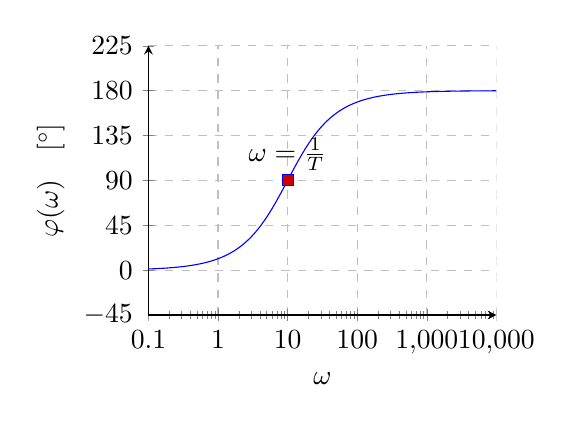
\begin{tikzpicture}
			            \begin{axis}[width=6cm,height=5cm,
					            axis lines = left,
					            xmode = log,
					            xlabel = \(\omega\), ylabel = {\(\varphi(\omega)\quad[^\circ]\)},
					            log ticks with fixed point,
					            xmin = 0.1, xmax = 10000,
					            ymin = -45, ymax = 225,
					            xtick = {0.1,1,10,100,1000,10000},
					            ytick distance = 45,
					            legend pos = north west,
					            ymajorgrids = true,
					            xmajorgrids = true,
					            grid style = dashed,
				            ]
				            \addplot [
					            domain=0.1:10000,
					            samples=200,
					            color=blue,
				            ] { 2*atan( x / 10 ) };
				            \addplot+ [color=blue] coordinates {
						            (10,90)
					            };
				            \node [above] at (axis cs: 10, 90) {$\omega=\frac{1}{T}$};
			            \end{axis}
		            \end{tikzpicture}
	            \end{center}
	      }
\end{itemize}


\end{document}